\documentclass[../../main.tex]{subfiles}

\graphicspath{{\subfix{../../immagini/}}}

\begin{document}
    Obiettivo di questo capitolo è di fornire una breve introduzione ai concetti fondamentali dell'apprendimento automatico con un interesse particolare per i concetti di \textit{apprendimento supervisionato}, applicandoli nello specifico alla \textit{classificazione} e alla \textit{regressione}.

    È utile iniziare riportando la formalizzazione del concetto di \textit{apprendimento} in ambito informatico data in \cite{Mitchell97}:
    
    ``Data una classe di problemi $T$ ed un metodo di misura delle prestazioni $P$ si dice che un generico programma apprende dall'esperienza accumulata in $T$ se le sue prestazioni, misurate tramite $P$, migliorano all'aumentare dell'esperienza $E$.'' 

    Nel contesto dei nostri esperimenti, ad esempio, il problema $T$ è quello di classificare correttamente, come phishing o legittimi, degli URL forniti in ingresso. Il programma migliorerà le proprie prestazioni $P$, misurate come abilità di discernere correttamente URL, grazie all'esperienza  $E$ guadagnata tramite l'osservazione di un elevato numero di URL di entrambe le categorie, imparando poi a generalizzare le caratteristiche principali di entrambe le tipologie di indirizzi e riuscendo infine a classificare correttamente  URL mai osservati in precedenza.

    In generale quindi possiamo definire un problema di apprendimento identificando tre proprietà: la classe del problema, la metrica per le prestazioni e la fonte dell'esperienza.

    Identificato un problema di apprendimento, l'obiettivo è ora quello di definire un approccio per la progettazione di sistemi in grado di risolvere tali problemi.

    Più in generale, è utile introdurre il concetto di agente, cioè un'entità in grado di percepire l'ambiente tramite sensori e di interagire con tale ambiente tramite degli attuatori. Possiamo definire diverse tipologie di agente a seconda di come questo lavora sulle percezioni ottenute dall'ambiente.

    \begin{figure}[H]
        \centering
        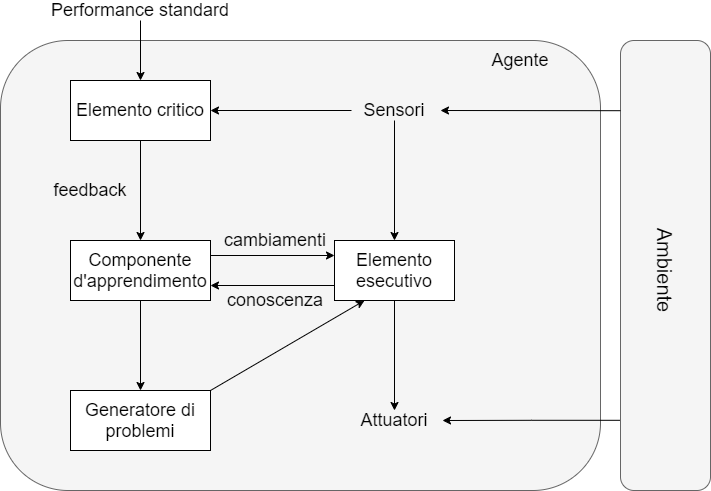
\includegraphics[width =\textwidth]{immagini/4_0/learning_agent.png}
        \caption{Schema di un learning agent.}
        \label{fig:learning_agent}
    \end{figure}

    Nello specifico, la tipologia di agente utilizzata nell'ambito dell'apprendimento automatico è quella che prende il nome di \textit{learning agent} (Figura \ref{fig:learning_agent}). Agenti di questo tipo possono essere suddivisi in quattro componenti principali, di cui i due più importanti sono il componente d'apprendimento, il cui compito è di migliorare le prestazioni dell'agente, e l'elemento esecutivo, il cui compito è di scegliere le azioni da compiere sulla base delle percezioni dall'ambiente. Il componente d'apprendimento quindi migliora l'agente, sulla base del feedback ricevuto dall'elemento critico, modificando il comportamento dell'elemento esecutivo.

    Si dice quindi che un agente apprende se le sue performance vanno a migliorare grazie a ripetute interazioni con l'ambiente in cui è inserito.
    È importante notare come il concetto di agente sia applicabile in generale a tutti i campi dell'intelligenza artificiale (\cite{russel2010}), non solo a quello del machine learning, trattato in questo capitolo.

    Possiamo definire diverse forme di apprendimento a seconda di come i vari componenti dell'agente vengono caratterizzati. Nello specifico, concentrandosi sulla tipologia di feedback ricevuto dall'agente vengono determinati le tre principali forme di apprendimento:
    
    \begin{itemize}
        \item apprendimento supervisionato: in questo caso l'agente apprende tramite un dataset di esempi, caratteristica fondamentale del dataset è il fatto che ad ognuno degli elementi è associata un'\textit{etichetta}, nei nostri esperimenti, ad esempio, ogni URL ha la relativa etichetta che indica la sua appartenenza ad  una delle due categorie. Più in generale, in problemi di apprendimento supervisionato ogni elemento deve apparire nella forma $ <\text{elemento}, \text{etichetta}> $.
        \item Apprendimento non supervisionato: a differenza di ciò che accade nel caso precedente, in questo contesto l'agente riesce ad apprendere senza avere un feedback con cui confrontare le proprie assunzioni. Esempio classico di apprendimento di questo tipo è il \textit{clustering}: il termine in generale si riferisce al raggruppamento di oggetti simili, dove il concetto di similarità dipende dal problema a cui ci si riferisce. Tipico esempio di algoritmo utilizzato in questo caso è k-means, intuitivamente l'algoritmo suddivide  l'insieme d'addestramento in $k$ cluster diversi, ognuno contenente elementi simili tra loro, l'algoritmo fornisce quindi una sorta di one-hot encoding $\boldsymbol{h}$ a k-dimensioni: se un elemento $\boldsymbol{x}$ appartiene ad un cluster $i$ allora $h_i = 1$, mentre tutti i rimanenti elementi del vettore saranno a 0 \cite{goodfellow2016deep}.
        \item Apprendimento semi-supervisionato: l'apprendimento avviene tramite un'insieme di esempi, di cui solamente una piccola parte possiedono un'etichetta fornita a priori, di fatto questa categoria di apprendimento cade nel mezzo tra i già citati apprendimento supervisionato e non supervisionato.
    \end{itemize}

    Altra forma di apprendimento che è importante menzionare è l'apprendimento per rinforzo: intuitivamente in problemi di questo tipo l'agente ha la possibilità di scegliere tra molteplici azioni, diverse a seconda dello stato in cui si trova, l'obiettivo è di riconoscere quali azioni in un determinato stato siano quelle che portano a massimizzare la reward ottenuta.\\
    Aspetto fondamentale è il fatto che per raggiungere questo obiettivo l'agente non abbia alcun indizio a priori sulla bontà delle azioni: è costretto a tentare diverse possibilità per scoprire quale sia la migliore, molto spesso la scelta di un'azione in uno stato porterà conseguenze non solo dirette, in termini di reward ottenuta, ma anche indirette, perché influenzerà le azioni possibili negli stati successivi.

    Questo tipologia di problemi si discosta quindi da quelli definiti sopra: nell'apprendimento supervisionato l'apprendimento avviene su un insieme di esempi legati alle relative etichette, queste forniscono già un'indicazione sull'azione migliore da compiere quando l'esempio si presenta all'agente, e l'obiettivo è quello di generalizzare: permettere all'agente di scegliere l'azioni migliori anche in esempi non presenti nell'insieme d'addestramento.\\
     Nell'apprendimento non supervisionato, seppur si lavori su dati senza etichette come nell'apprendimento per rinforzo, il fine è di apprendere gli eventuali pattern presenti negli insiemi di dati su cui si lavora, non di trovare l'azione migliore \cite{Sutton1998}. 

    Ci concentriamo ora sull'apprendimento supervisionato, che sarà la tipologia di apprendimento che sfrutteremo negli esperimenti descritti nel capitolo \ref{chap:Esperimenti}.
    


\end{document}